Teknik dasar dari route planning adalah menggunakan algoritma Dijkstra (\cite{Dijkstra59}), algoritma Djikstra mempertahankan \textit{priority queue} $Q$ dari simpul-simpul diurutkan berdasarkan berdasarkan jarak tentatif dari s. Algoritma menginisialisasi semua jarak dengan nilai tak terhingga, kecuali jarak simpul asal $s$ ke simpul asal $s$ yang nilainya sama dengan 0, dan menambahkan $s$ ke $Q$. Pada setiap iterasi, ekstrak simpul $u$ dengan jarak paling kecil dari $Q$ dan pindai semua sisi $a=(u,v) \in A$ yang bersisian dengan $u$. Untuk semua sisi, tentukan jarak ke $v$ melalui sisi $a$ dengna menghitung $dist(s,u) + l(a)$. Jika nilai dari $dist(s,u) + l(a)$ lebih kecil, lakukan relaksasi sisi: perbarui jarak $v$ dari $s$ dan tambahkan simpul $v$ dengan jarak baru ke $Q$. Algoritma dijkstra memiliki kompleksitas waktu $O((|V|+|A|)log|V|)$ dengan binary heap, dan jika menggunakan Fibonnaci heap kompleksitas waktu menjadi $O(|A|+|V|log|V|)$. Meskipun efisien untuk jaringan berukuran sedang, kinerjanya menurun untuk jaringan jalan berskala besar (seperti pada jaringan transportasi) karena menjelajahi ruang pencarian yang besar. Eksperimen yang dilakukan pada penelitian oleh \cite{Bast2015}, pada graf jaringan jalan Eropa Barat dengan 18 juta simpul dan 42.5 juta sisi, algoritma dijkstra menjawab kueri dalam 2.195 detik, yang mana tidak cocok untuk aplikasi navigasi \textit{real-time}. Dalam praktiknya, kita dapat mempersempit ruang pencarian dengan melakukan \textit{bidirectional search}. \textit{Bidirectional search} berjalan secara bersamaan dengan \textit{forward search} dari $s$ dan \textit{backward search} dari $t$. Algoritma akan berhenti ketika perpotongan dari kedua ruang pencarian mengandung simpul $x$ yang tereletak pada rute terpendek dari $s$ ke $t$. Untuk jaringan jalan, \textit{bidirectional search} mengunjungi sekitar setengah jumlah simpul dari \textit{unidirectional search}.

Algoritma dasar tersebut dapat ditingkatkan dengan memfokuskan pencarian ke arah target, bukan memindai simpul-simpul di dekatnya secara menyeluruh, teknik ini dinamakan sebagai \textit{Goal Directed Search}. Salah satu algoritma dari teknik \textit{goal-directed search} adalah algoritma $A^*$. $A^*$ menggunakan fungsi potensial $\pi:V->\mathbb{R}$ dengan syarat $l(v,w)-\pi(v)+\pi(w)\ge0$ for $(v,w)\in E$ pada setiap simpul, yang mana adalah batas bawah dari $dist(u,t)$ dari $u$ ke $t$. Lalu menjalankan algoritma dijkstra dengan prioritas dari simpul $u$ ditetapkan menjadi $dist(s,u)+\pi(u)$. Hal ini menyebabkan algoritma memindai simpul-simpul yang lebih dekat dengan target $t$ dipindai lebih awal. Untuk mengadaptasi \textit{bidirectional search} pada algoritma $A^*$, tetapkan fungsi potensial untuk \textit{forward search} sebagai $(\pi_f-\pi_r)/2$ dan fungsi potensial untuk \textit{backward search} sebagai $(\pi_r-\pi_f)/2$. Sayangnya, untuk jaringan jalan dengan fungsi potensial ditetapkan sebagai jarak geografis antara $u$ dan $t$ dibagi dengan kecepatan travel maksimum, peningkatan kinerja dari algoritma A* sangat kecil, pada penelitian oleh \cite{Goldberg2005}, kueri algoritma $A^*$ pada graf jaringan jalan dengan 2 juta simpul dan 5 juta sisi diselesaikan dalam hitungan waktu 1.2 detik. Penelitian oleh \cite{Goldberg2005} mempercepat algoritma $A^*$ dengan menggunakan batas bawah yang jauh lebih baik, algoritma ini dinamakan dengan $ALT(A^*,landmarks, and \ triangle \ inequality)$. Dalam fase praproses, teknik ini memilih himpunan $L\subseteq V$ \textit{landmarks} dan menyimpan jarak antara \textit{landmarks} dan semua simpul di dalam graf. Setiap \textit{landmark} $l_i$, ketidaksamaan segitiga $\text{dist}(u,t)+\text{dist}(t,l_i)\geq\text{dist}(u,l_i)$ dan $\text{dist}(u,t)+\text{dist}(l_i,u)\geq\text{dist}(l_i,t)$ harus terpenuhi. Selama kueri $s-t$, ALT menggunakan fungsi potensial $\pi_t=\max_{l \in L} \Big\{ | \text{dist}(l,t)-\text{dist}(l,v)|,|\text{dist}(v,l)-\text{dist}(t,l)|\Big\}$. Lihat Gambar~\ref{fig:alt-triangle-ineq} untuk ilustrasi dari ketidaksamaan segitiga untuk ALT. Teknik ALT berhasil meningkatkan performa dari algoritma $A^*$, dimana pada penelitian oleh \cite{Goldberg2005} kueri pada graf dengan 2 juta simpul dan 5 juta sisi dapat diselesaikan dalam hitungan waktu 40 milidetik. Teknik \textit{goal-directed search} lain adalah Arc Flags (\cite{Kohler2005}), pada fase praproses, graf di partisi menjadi sejumlah K sel yang memiliki jumlah simpul yang mirip dan jumlah simpul batas yang sedikit. Setiap sisi menyimpan larik dengan elemen bit dan ukuran k, dimana bit ke-i ditetapkan ke 1 jika sisi terletak pada jalur terpendek menuju suatu simpul pada sel i. Pada fase kueri, algoritma memangkas sisi yang tidak memliki nilai bit sama dengan 1 untuk sel yang berisi simpul t. Untuk membuat \textit{arc flags} untuk setiap sel, algoritma menumbuhkan pohon jalur terpendek mundur (berlawanan dengan rute terpendek) dari setiap simpul batas (dari sel-i), dan menentapkan \textit{flag} ke-i untuk setiap sisi dari pohon. Teknik Arc Flags dapat menjawab kueri acak pada graf jaringan jalan Eropa Barat dengan 18 juta simpul dan 42.5 juta sisi dengan hitungan waktu 0.408 milidetik (\cite{Bast2015}).

\begin{figure}[H]
    \centering
    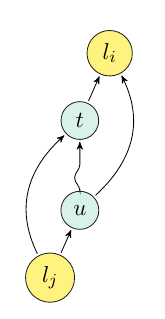
\includegraphics[]{figures/ALT.png}
    \caption{ketidaksamaan segitiga untuk ALT (diadaptasi dari~\cite{Bast2015}).}
    \label{fig:alt-triangle-ineq}
\end{figure}

Teknik akselerasi lain adalah dengan menggunakan teknik \textit{Separator-Based}. Teknik ini memanfaatkan fakta bahwa jaringan jalan dapat dibagi menjadi wilayah-wilayah yang lebih kecil dan seimbang (sel-sel) yang dipisahkan oleh sekumpulan titik simpul atau sisi, yang disebut sebagai pemisah. Teknik High-Performance Multilevel Routing (\cite{DellingHPML}) memanfaatkan \textit{vertex separators}, yaitu subset simpul-simpul $S\subset V$ yang mana penghapusannya mengurai graf menjadi beberapa sel, dan proses pembuatan partisi dilakukan secara rekursif pada setiap sel sehingga menghasilkan $multilevel \ overlay \ graph$. Fase praproses dari teknik ini dimulai dengan memilih subset $S$ lalu mempartisi graf jaringan jalan dengan menggunakan subset tersebut. Lalu, untuk setiap simpul $u,v\in S$, sebuah sisi $(u,v)$ ditambahkan ke graf \textit{overlay} $G'$ jika rute terpendek dari $u$ dan $v$ tidak mengandung simpul $w\in S$. Teknik ini juga menambahkan sisi dari simpul pemisah pada level $i$ dan simpul-simpul pemisah pada level $(i-1)$. Lihat Gambar~\ref{fig:hpml} untuk ilustrasi. Teknik HPML dapat menjawab kueri acak pada graf jaringan jalan Eropa Barat dengan 18 juta simpul dan 42.5 juta sisi dengan hitungan waktu 0.01 milidetik (\cite{Bast2015}). Teknik lain dari \textit{separator-based techniques} adalah Customizable Route Planning (CRP) (\cite{Delling2015}). Pada fase praproses, teknik ini melakukan partisi graf hingga menghasilkan graf \textit{overlay} $\mathcal{H}=(C_1,\ldots,C_k)$ dari simpul-simpul awal graf menjadi sel-sel seimbang yang menimalkan jumlah dari sisi potong (yang menghubungkan simpul-simpul batas yang terletak pada sel yang berbeda). Sisi-sisi jalan pintas yang menghubungkan antara titik-titik batas (yang merupakan rute terpendek dari setiap pasang simpul batas) dalam setiap sel ditambahkan pada graph \textit{overlay}. Lihat Gambar~\ref{fig:crp-overlay} untuk ilustrasi graf \textit{overlay} menggunakan CRP. Pada fase kustomisasi, bobot dari setiap sisi jalan pintas dihitung dengan menggunakan algoritma dijkstra yang dijalankan secara paralel pada setiap simpul batas, hal ini memungkinkan pembaruan bobot pada sisi-sisi graf menyesuaikan pembaruan kondisi lalu lintas. Algoritma kueri kemudian menjalankan algoritma Dijkstra pada subgraf yang diinduksi oleh sel yang berisi s dan t ditambah dengan graf \textit{overlay}. Teknik CRP dapat menjawab kueri acak pada graf jaringan jalan Eropa Barat dengan 18 juta simpul dan 42.5 juta sisi dengan hitungan waktu 1.65 milidetik (\cite{Delling2015}).


\begin{figure}[H]
    \centering
    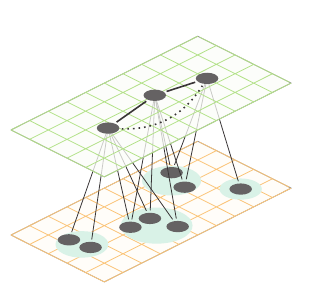
\includegraphics[]{figures/HPML.png}
    \caption{Sisi-sisi jalan pintas pada High-Performance Multilevel Routing (diadaptasi dari~\cite{Bast2015}).}
    \label{fig:hpml}
\end{figure}


\begin{figure}[H]
    \centering
    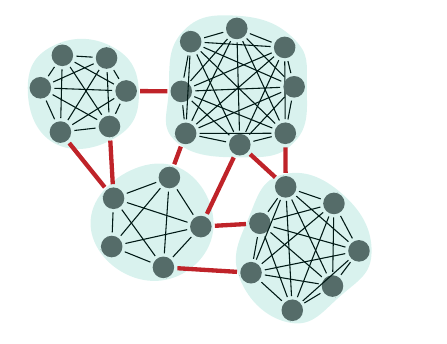
\includegraphics[]{figures/CRP.png}
    \caption{graf \textit{overlay} hasil fase kustomisasi CRP (diadaptasi dari~\cite{Bast2015}).}
    \label{fig:crp-overlay}
\end{figure}

Hierarchical techniques memanfaatkan hierarki jaringan jalan untuk mempercepat pencarian rute terpendek. Dalam jaringan jalan di dunia nyata, rute yang cukup panjang cenderung menyatu menjadi serangkaian jalan arteri yang lebih kecil, seperti jalan raya, yang berfungsi sebagai jalan utama dari perjalanan jarak jauh. Dengan memanfaatkan struktur ini, metode hierarki mengurangi ruang pencarian dengan berfokus pada simpul dan sisi dengan prioritas tinggi. Salah satu algoritma yang menggunakan teknik ini adalah \textit{Contraction Hierarchies} (CH), yang diperkenalkan pada penelitian oleh \cite{Geisberger2012}. Algoritma ini beroperasi dalam dua tahap: prapemrosesan dan kueri. Selama prapemrosesan, simpul-simpul diurutkan berdasarkan prioritasnya dan setiap simpul akan dikontraksi. Untuk mengkontraksi simpul $v$, simpul $v$ dihapus (untuk sementara) dari graf, dan sisi jalan pintas akan dibuat diantara setiap pasangan $u, w$ dari simpul yang bersebelahan dengan $v$ jika jalur terpendek dari $u$ dan $w$ unik dan mengandung simpul $v$. Pada fase kueri, pencarian dua arah dijalankan dari sumber dan target, tetapi dibatasi pada sisi yang mengarah ke simpul berperingkat lebih tinggi. Lihat Gambar~\ref{fig:query-ch} untuk ilustrasi kueri \textit{Contraction Hierarchies}. Misalkan $d_s(u)$ dan $d_t(u)$ adalah label jarak dari pencarian maju dan pencarian mundur. Oleh karena itu, di antara semua simpul $u$ yang dikunjungi oleh kedua pencarian, simpul yang meminimalkan $d_s(u)$ +  $d_t(u)$ mewakili jalur terpendek. Kueri rute terpendek dari algoritma \textit{Contraction Hierarchies} dapat dijawab dalam hitungan waktu 0.152 milidetik (\cite{Geisberger2012}). Metode hierarki lainnya adalah algoritma Reach (\cite{Gutman2004}), Reach mendefinisikan ukuran sentralitas untuk simpul berdasarkan seberapa jauh suatu simpul berada di sepanjang jalur terpendek. Misalkan $P$ adalah lintasan $s–t$ terpendek yang memuat simpul $u$. Reach $r(u,P)$ dari simpul $u$ terhadap $P$ didefinisikan sebagai $min\{dist(s,u), dist(u,t)\}$. Reach global dari simpul $u$ pada graf $G$ adalah \textit{reach} maksimum dari $u$ pada semua semua jalur terpendek yang memuat $u$. Kueri s-t algoritma reach menjalankan algoritma dijkstra, tetapi memangkas pencarian di setiap simpul $u$ yang memiliki $dist(s,u)>r(u)$ dan $dist(u,t)>r(u)$. Nilai \textit{reach} dihitung pada fase prapemrosesan dengan cara menghitung jalur terpendek untuk semua pasangan simpul. Kueri rute terpendek dari algoritma Reach dapat dijawab dalam hitungan waktu 0.152 milidetik (\cite{Bast2015}).


\begin{figure}[H]
    \centering
    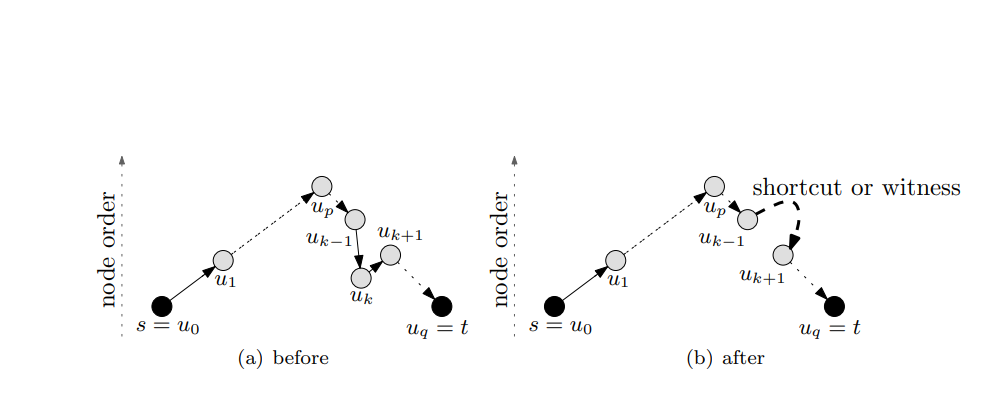
\includegraphics[width=\linewidth, keepaspectratio]{figures/CH.png}
    \caption{Ilustrasi kueri \textit{Contraction Hierarchies} (diadaptasi dari~\cite{Geisberger2012}).}
    \label{fig:query-ch}
\end{figure}


Teknik akselerasi lainnya adalah \textit{Bounded-Hop Techniques}.Ide dari teknik \textit{bounded-hop} adalah menghitung jarak antar pasangan simpul terlebih dahulu, secara implisit menambahkan "jalan pintas virtual" ke graf. Kueri kemudian dapat mengembalikan panjang jalur virtual dengan sangat sedikit \textit{hop}. Pada fase prapemrosesan, label $L(u)$ yang berisi sekumpulan simpul (\textit{hub} dari $u$) beserta jaraknya dari $u$ dihitung untuk setiap simpul $u$ pada graf, sehingga untuk setiap pasangan simpul $u,v$ jarak $dist(u,v)$ dapat ditentukan dengan melihat label $L(u)$ dan $L(v)$. pada Algoritma \textit{Hub Labelling} (HL) (\cite{Abraham2011}), \textit{hub} dari $u$ dipilih sedemikian rupa sehingga memenuhi properti \textit{cover}: untuk setiap pasang simpul $(s,t)$, $L(s)\cap L(t)$ harus memuat setidaknya satu simpul pada jalur terpendek $s-t$. Jarak dari $dist(s,t)$ dapat dihitung secara linear dengan menghitung $dist(s,t) = \min \{ dist(s,u) + dist(u,t) \mid u \in L(s) \ \text{dan} \ u \in L(t) \}$. Kueri menggunakan algoritma \textit{Hub-Labelling} dapat dijawab dalam hitungan 0.00056 milidetik. Algoritma kedua dari teknik \textit{Bounded-Hop} adalah \textit{Transit Node routing} (TNR) (\cite{Arz2013}). Ide utama dari algoritma TNR adalah memilih sejumlah simpul transit $T\subseteq V$ dan menghitung semua jarak berpasangan di antara simpul-simpul tersebut, lalu buat himpunan simpul akses $A(u)=\{v \mid v\in T \land \  v \text{ adalah adalah simpul transit pertama yang terletak pada jalur terpendek } P \text{ dari } u  \}  \subseteq T$ dari setiap simpul $u \in V \setminus T$. Pada fase kueri, algoritma ini menggunakan tabel jarak untuk memlilih rute yang meminimalkan jarak $a(s)-a(t)-t$, dimana $a(s)\in A(s) \text{ dan } a(t) \in A(t)$ adalah simpul akses. Kueri menggunakan algoritma \textit{Transit Node Routing} dapat dijawab dalam hitungan 0.00327 milidetik. Algoritma ini dapat menghasilkan hasil kueri yang tidak benar jika jalur rute terependek tidak memuat simpul dari $T$. Untuk mengatasi masalah tersebut, dibuatlah \textit{locality filter} yang memutuskan apakah kueri mengandung simpul dari $T$, jika kueri tidak mengandung simpul dari $T$ maka algoritma ini kembali menggunakan algoritma akselerasi lain seperti Contraction Hierarchies. Secara umum, teknik \textit{bounded-hop} mencapai waktu kueri yang sangat cepat (bahkan lebih cepat dibandingkan metode hierarki), tetapi dengan biaya praproses dan penggunaan memori yang relatif tinggi. Oleh karena itu, teknik ini sangat cocok untuk aplikasi navigasi statis berskala besar, namun kurang fleksibel pada skenario jaringan jalan yang sangat dinamis. Tabel 2.1 menunjukkan performa dari beebrapa teknik akselerasi dari seribu kueri yang dihasilkan secara acak pada jaringan jalan Eropa Barat.

